%#! platex main.tex
\documentclass[a4paper,12pt]{jreport}
\usepackage{jgraduate}          % 卒論・修論用スタイル

%% 索引作成
%\usepackage{makeidx}
% dvipdfmxを使用しない場合はオプションを変更すること
\usepackage[dvipdfmx]{graphicx}
% 数字付きリストでラベルを使う
\usepackage{enumerate}
% 数学記号など
\usepackage{amsmath}
\usepackage{amssymb}
\usepackage{amsthm}
% URLをいい感じにする
\usepackage{url}
\usepackage{cite}

%------------------------------
% 余白設定
%------------------------------
\usepackage[left=27mm,right=27mm,top=45mm,bottom=45mm,%
 headheight=5mm,headsep=10mm,%
 footskip=12mm%
 ]{geometry}

%------------------------------
% hyperref
%  日本語の文字コード設定が分からない人はコメントアウトすること.
%------------------------------
% PDF化したときにしおりが作成され,図表へのジャンプも可能となる.
\usepackage{atbegshi}
% Mac/Linuxの場合
%   ※Ubuntuの場合はEUC-UCS2を自分で入れないとダメ.
\AtBeginShipoutFirst{\special{pdf:tounicode EUC-UCS2}}
%% Winの場合
%\AtBeginShipoutFirst{\special{pdf:tounicode 90ms-RKSJ-UCS2}}
% 以下は共通
\usepackage[dvipdfm,a4paper,bookmarks,bookmarksnumbered,%
 hidelinks,% 目次やリンクテキストの周囲の赤枠を消す
 bookmarksopen=false,pdfstartview={FitH},%
 bookmarkstype=toc,%
 setpagesize=false,%
 pdfauthor={大平 祐大},%
% setpagesize=false,% PDFのサイズがおかしい場合はこれを有効化
 pdftitle={master_thesis}]{hyperref}

%----------------------------------------------------------------------
% 設定
%----------------------------------------------------------------------
% 目次の深さはsubsubsectionまで
\setcounter{tocdepth}{3}

% 基準となる図の幅
\newlength\figurewidth
\setlength{\figurewidth}{0.8\textwidth}
% 縦に並べた図の間の基準となるスペース
\newlength\figuresep
\setlength{\figuresep}{0.8\floatsep}

%----------------------------------------------------------------------
% 文書基本情報
%----------------------------------------------------------------------
% タイトル
\title{イアラブルデバイスのマイクを用いた\\食事内容と咀嚼回数の推定手法の提案}

% 著者
\author{大平 祐大}

% 所属
\university{九州大学大学院}
\department{システム情報科学府}
\course{修士課程}
\major{情報理工学専攻}
% \submajor{情報理工学コース}

% 提出日(月までを書く)
\date{令和6年2月}

%% 書いている途中では以下のようにしておくと一部だけをタイプセットできる
% \includeonly{intro}

%======================================================================
% テキスト開始
%======================================================================
\begin{document}
% 表紙
\maketitle
% 表紙はページ番号を出力しない
\thispagestyle{empty}

%----------------------------------------------------------------------
% 概要
%----------------------------------------------------------------------
\begin{abstract}
    食事管理アプリケーションの登場により食品名やカロリーの自動記録が可能になっているが, 健康管理の観点では, 食べる順番, 食べる速度, 咀嚼の回数といった食べ方の情報も重要な要素である. このような食事過程のセンシングを試みる先行研究は存在するが, 独自に開発された専用デバイスの装着が必要不可欠であり, その普及には課題が残っている. そこで, 本研究ではすでに普及している市販のイヤラブルデバイスとスマートフォンのみを使用し, 食事内容と咀嚼回数の推定が可能なセンシング手法を提案する. 具体的には, 食事中に発生する音をメルスペクトログラムに変換し, 畳み込みニューラルネットワークで学習させ, 食事内容推定モデルの作成を行う. また, メルスペクトログラムの各時間軸毎の全ての周波数帯の信号強度の平均をとり, ピーク検出を行うことで咀嚼の検出を行う. 本研究では, データ収集のために, 食事中に発生する音を録音しつつ, 被験者自身が咀嚼回数をカウントできる独自のアプリケーションを開発した. データ収集実験では, 15名の被験者を対象にアプリケーションを配布し, ワイヤレスイヤホンを装着した状態で, 一品ずつ食事を行った. また, 咀嚼検出の分析のために, 実験中に被験者自身の咀嚼回数をカウントするように指示した. 16種類の食品に対して録音を行い, 合計で13422秒の音データを得られた. その結果, 収集した音データで食事内容推定モデルを学習させたところ, 検証用の音データに対して, 精度$77.5\%$で食事内容を推定できることを確認した. また, 10秒間の音データに対して被験者がカウントした咀嚼回数とピーク検出回数との間の平均絶対値誤差$MAE$を算出したところ, $MAE = 4.9$を確認することができた.
\end{abstract}

%----------------------------------------------------------------------
% 目次のページ番号は1から
\setcounter{page}{0}
% 目次
\tableofcontents

% 本文のページ番号はアラビア数字
\pagenumbering{arabic}

%======================================================================
% 本文ここから
%======================================================================

% 章ごとのファイルを読み込む
% YaTeXなら各ファイルを読み込む行でC-c gでジャンプできる
%#! platex main.tex

\chapter{はじめに}
\label{cha:intro}

近年, 食事管理アプリにより, 食事の写真から食品やカロリなどの栄養素を自動で記録できるようになってきた. これらの技術は, 食事の写真から画像認識技術により, 食品を特定し, 栄養データを算出することがベースとなっている. 例えば, カロミル\footnote{健康管理アプリ、カロミルとは?|食事内容・日々の体重・運動量をアプリで簡単に記録~\url{https://www.calomeal.com/about-calomeal/}}は, iOS・Androidアプリとして提供されており, スマートフォンのカメラで食事の写真を撮るだけで, 食事の内容を解析し, 自動で摂取栄養素を記録することができる.

一方で, 健康的な食事を行う上で, 摂取栄養素だけでなく食べる順番やスピードを意識することは非常に重要である. 日本の学校教育では, 米やパンなどといった主食と, 汁物や飲料, おかずとを順序よく食べる方法「三角食べ」を推奨していた. 学術面においても, 食べる順番に重点をおいた食事指導の有効性については関西電力医学研究所の研究グループにより証明されており, 最初の5分間は食物繊維を含む食品やタンパク質や脂質を含む食品を食べ, その後, 炭水化物を含む食品を, 食物繊維を含む食品やタンパク質や脂質を含む食品と一緒に食べるよう指導すると, 体重の減量に影響を与えることを報告した\cite{yabe2019107450}. さらに, 糖尿病予防にも効果があり, 野菜から先に摂取すると, 米飯から先に摂取した場合と比較して食後の血糖値の上昇を抑えることができる\cite{tonyobyo53112}. また, 食べる速度についても, 早食いは肥満や糖尿病, 心臓に対して悪影響を及ぼすことが明らかになっている\cite{20249}\cite{beyond_willpower}. 一品ずつ集中して食べる「ばっかり食べ」や咀嚼をあまり行わない「早食い」をする子供に対して注意することは妥当であると言える.

%%%%%%%%%%%%%%%%%%%%%%%%%%%%%%%%%%%%%%%%%%%%%%%%
\begin{figure}[t]
  \begin{center}
    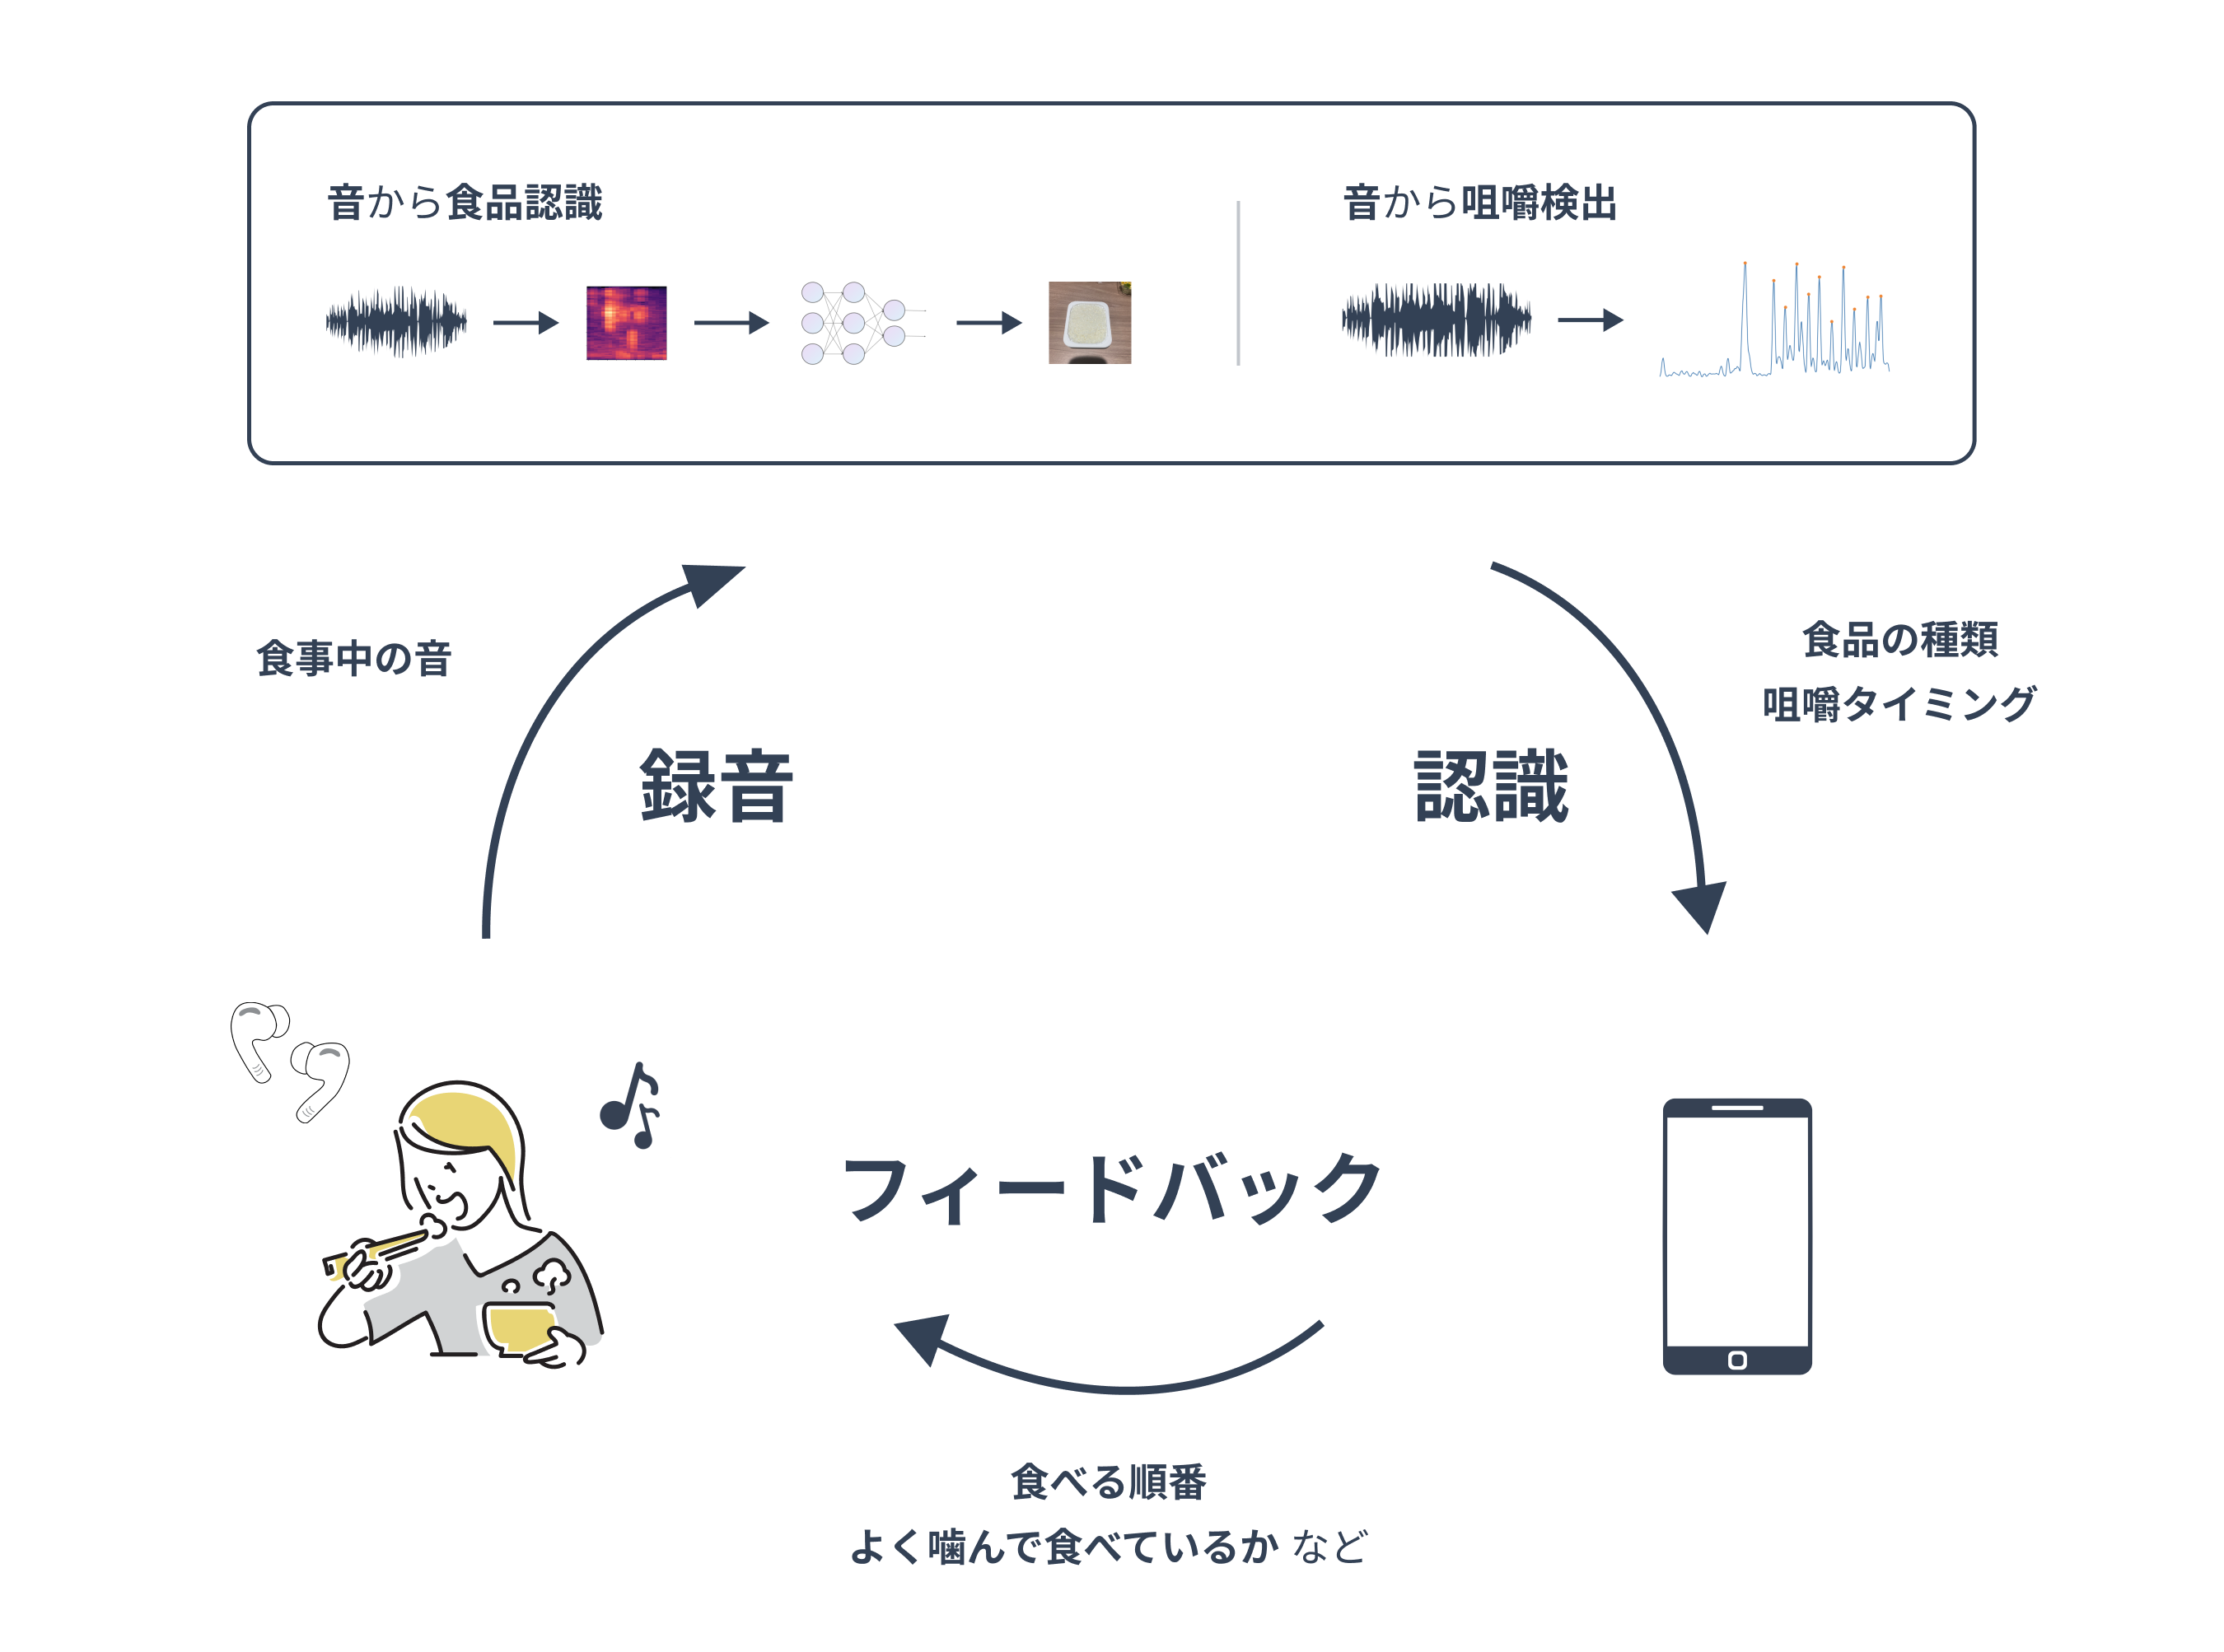
\includegraphics[clip,  width=1.0\hsize]{img/system.png}
    \caption{食事中の音を分析するための計測システムの提案}
    \label{fig:system}
  \end{center}
\end{figure}
%%%%%%%%%%%%%%%%%%%%%%%%%%%%%%%%%%%%%%%%%%%%%%%%

食べる順番や速度などを含む食事行動の記録に着目した研究や技術も存在する. シャープが開発したbitescan\footnote{咀嚼計「bitescan(バイトスキャン)」:シャープ~\url{https://jp.sharp/business/bitescan/}}では, 独自の耳掛け式のウェアラブルデバイスを用いて, 食事中にリアルタイムで咀嚼回数を計測することで, 咀嚼テンポや食事の時間などを記録することができる. しかし, 独自のウェアラブルデバイスが必要となるため, 誰でも利用できるアプリケーションに組み込むことは難しく, そもそも咀嚼回数のみを計測しているため, 食べる順番を記録することができない. また, 食べる順番や速度などをアドバイスするために, ウェアラブルデバイスで食事行動を撮影した一人称映像から食事内容をリアルタイムで検出する研究も存在する\cite{10.1145/3551626.3564964}. しかし, この手法も食事中にカメラで撮影し続ける必要があるため, 一般的な食事シーンで計測を行うのは受け入れ難い.

我々の研究グループでは, 健康的な食生活を促進する行動変容支援システムとしてeat2picを提案している\cite{10.1145/3580784}. しかし, eat2picのセンシングアプローチは, カメラとIMUを搭載した専用の箸型センサを使用する必要があるため, 日常生活での利便性や社会全体への普及可能性という観点で, 課題が残っている. それに対して, 本研究ではすでに普及している市販のイヤラブルデバイスとスマートフォンのみを使用し, 食事内容と咀嚼回数の推定が可能なセンシング手法を提案する. 本稿では, 図\ref{fig:system}に示すように, 食事中に発生する音を収集し, 収集したデータを分析し, 食事内容と咀嚼回数の推定を行う一連の設計について述べる. 図\ref{fig:system}では, 計測・分析・可視化というステップを示しているが, 本稿では計測・分析のみを行い, 可視化については本稿では取り扱わない. 具体的には, 食事中の音をワイヤレスイヤホンで録音しつつ, 被験者自身が咀嚼回数をカウントできる独自のアプリケーションを開発し, このアプリケーションを用いてデータ収集を行う. 分析については, 計測した食事中の音をメルスペクトログラムに変換し, 畳み込みニューラルネットワークで学習させ, 食事内容推定モデルの作成を行う. また, メルスペクトログラムの各時間軸毎の全ての周波数の信号強度の平均をとり, ピーク検出を行うことで咀嚼の検出を行う. データ収集実験では, 15名の被験者を対象にアプリケーションを配布し, ワイヤレスイヤホンを装着した状態で, 一品ずつ食事を行った. また, 咀嚼検出の分析のために, 実験中に被験者自身の咀嚼回数をカウントするように指示した. 16種類の食品に対して録音を行い, 合計で13422秒の音データを得られた. その結果, 収集した音データで食事内容推定モデルを学習させたところ, 検証用の音データに対して, 精度$77.5\%$で食事内容を推定できることを確認した. また, 10秒間の音データに対して被験者がカウントした咀嚼回数とピーク検出回数との間の平均絶対値誤差$MAE$を算出したところ, $MAE = 4.9$を確認することができた.

本稿の構成は以下の通りである.
第2章で食事内容の推定に関する関連研究について述べる. 第3章でデータ収集アプリケーションの設計・開発について述べ,第4章で食事中の音から食事内容・咀嚼回数を推定する手法について述べる. 第5章で評価実験について述べ,最後に第6章で本稿の結論および今後の課題について述べる.

%#! platex main.tex

%======================================================================
\chapter{関連研究}
\label{cha:research}

本章では, 食品認識に関する関連研究\ref{related_work}について述べたあと, 本研究の手法であるイヤラブルデバイスを用いたHARについて言及する.

\begin{table*}[t]
    \centering
    \caption{食品認識に関する関連研究}
    \label{related_work}
    \scalebox{0.9}{
        \begin{tabular}{c|c|c|c}
            \hline
            \textbf{年度} & \textbf{参考文献}                  & \textbf{手法}                 & \textbf{使用するデバイス}   \\ \hline\hline
            2017        & \cite{10.1145/3063592}         & 食事の画像から推定                   & カメラ(スマートフォン)        \\ \hline
            2019        & \cite{1523669555317207552}     & \begin{tabular}{c}パンの画像から種類を識別し, \\パン専用のレジとして応用\end{tabular} & 独自のレジ装置             \\ \hline
            2022        & \cite{10.1145/3551626.3564964} & 食事中の一人称映像から時系列毎に検出          & カメラ                 \\ \hline
            2022        & \cite{app12126135}             & 食事中の気管下部から皮膚の動きから推定         & \begin{tabular}{c}独自のネックレス型の\\ウェアラブルセンサ\end{tabular} \\ \hline
            2023        & 提案手法                           & 食事中に発生する音から推定               & \begin{tabular}{c}マイクを搭載した\\イヤラブルデバイス \end{tabular}  \\ \hline
        \end{tabular}
    }
\end{table*}

%----------------------------------------------------------------------
\section{食品認識}

食品認識における関連研究の中で, (1)食事の画像から食品を推定する手法, (2)ユーザ自身の食事行動を撮影した一人称の動画から時系列順で食品推定を行う手法, (3)独自のウェアラブルデバイスを用いて計測したセンサデータを元に食品推定を行う手法について述べる.

%----------------------------------------------------------------------
\subsection{画像ベース}

画像を利用した分析手法は, 食品認識において最も基本的な手法で, 近年では特にディープラーニングによる画像認識手法が主流となりつつある\cite{10.1145/3063592}. また, 実際の食事管理アプリケーションにもすでに広く統合されており, 食事メニューの推定だけでなく, そこから摂取栄養素を記録することができる. その他にも応用例として, パンの画像から種類を識別するパン画像認識レジ「BakeryScan」というものまで存在する\cite{1523669555317207552}. しかし, 画像は非時系列データなので, リアルタイムでの食事内容の推定には向かないという問題点が存在する.

%----------------------------------------------------------------------
\subsection{動画ベース}

動画を利用した分析手法は, 先ほど取り上げた画像ベースの手法の応用例となっており, ウェアラブルカメラで撮影した食事中の一人称映像をフレームに分割することで, 時系列順に食事内容の推定を行うことができる\cite{10.1145/3551626.3564964}. しかし, 食事の様子を常にカメラで撮影し続ける必要があるため, 一般的な食事シーンにおいては受け入れ難いという問題点が存在する.

%----------------------------------------------------------------------
\subsection{センサベース}

センサデータは時系列データであるため, 食事内容をリアルタイムで検出することができる. 独自のウェアラブルデバイスを用いた手法として, 食事中の気管下部から皮膚の動きを検出する圧電センサを組み込んだネックレス型のウェアラブルセンサが存在する\cite{app12126135}. しかしながら, 独自のウェアラブルデバイスの形状によっては, 一般的な食事シーンにおいて着用が難しく, そもそも独自のウェアラブルデバイスを普及させる必要がある.

%----------------------------------------------------------------------
\section{イヤラブルデバイスを用いたHAR}

近年, イヤラブルなデバイスを用いたHuman Activity Recognition(HAR)に関する研究が活発に行われてきている. 本章では, 一般的なハイエンドなワイヤレスイヤホンに搭載されている慣性計測ユニット(IMU)を用いた手法と従来のワイヤレスイヤホンにも搭載されているマイクを用いた手法について述べる.

%----------------------------------------------------------------------
\subsection{IMUベース}

IMUを搭載したウェアラブルデバイスを耳に装着することで, 特に頭の動きを認識することができる. Tahera HossainらはIMUを搭載したワイヤレスイヤホンを用いて, 頭や口に関連する行動である6つの活動(話す・食べる・首を振る・頷く・とどまる・歩く)を分類する手法を提案している\cite{10.1145/3341162.3343822}. また, Dhruv VermaらもIMUを搭載した市販のワイヤレスイヤホンを用いて, 46種類の表情を認識するExpressEarというシステムを提案している\cite{10.1145/3478085}.

%----------------------------------------------------------------------
\subsection{マイクベース}

マイクを用いた手法は, 非常に多種多様な研究が存在する. Yuntao Wangらは, イヤホンを用いた音響測距に基づく新しい顔追跡技術であるFaceOriを提案している\cite{10.1145/3491102.3517698}. また, Xuhai Xuらは, 市販のワイヤレスイヤホンのマイクから顔周りのジェスチャを検出し, さらにジェスチャからスマートフォンを操作できるEarBuddyというシステムを提案している\cite{10.1145/3313831.3376836}. また, 歯のジェスチャを行う際に発生する音波をユーザー認証に活用するといった変わった研究も存在する\cite{10.1145/3460120.3485340}.

イヤラブルデバイスのマイクは, 特に口から発生する音を捕捉することができるため, 本研究でもこのアプローチを採用する.

%%% Local Variables:
%%% mode: yatex
%%% TeX-master: "main"
%%% End:

%#! platex main.tex

%======================================================================
\chapter{おわりに}
\label{cha:conclu}

%----------------------------------------------------------------------
\section{本研究の主たる成果}
\label{sec:main-result}

何もねぇ...

本当にねぇ...

%----------------------------------------------------------------------
\section{今後の課題}
\label{sec:future}

課題なんてあろうか.
いや,あるわけがない.
全てが終わったのだから.


% 以下はRefTeX用
%%% Local Variables:
%%% mode: yatex
%%% TeX-master: "main"
%%% End:


% 謝辞
%#! platex main.tex
%======================================================================
% 謝辞
%======================================================================
\acknowledgment

本研究の機会を与えてくださり, 様々なご指導を頂きました九州大学大学院システム
情報科学研究院の荒川豊教授に深く感謝いたします. 本研究をすすめるにあたり, 多く
のご助言とご協力を頂きました九州大学大学院システム情報科学研究院の中村優吾助教
に深く御礼申し上げます. 最後に, 日頃の研究活動において様々なご協力, ご助言を頂きました, 九州大学大学院システム情報科学研究院荒川・峯研究室諸氏に深く感謝し,
御礼を申し上げます.


%----------------------------------------------------------------------
% 参考文献
%----------------------------------------------------------------------
\bibliographystyle{sieicej}
\bibliography{bib/IEEEfull,bib/mystr_IEEEfull,bib/my,bib/pub}
% 書き終えたら,↑の2行をコメントアウトして,BibTeXが生成したmain.bbl
% をref.texという名前に変更して
% ↓を有効化するとよい.必要があれば手動で修正する.
%\include{ref}

%----------------------------------------------------------------------
% 発表文献
%----------------------------------------------------------------------
%#!platex main.tex
%======================================================================
% Publications
%======================================================================
\publications

% 数が少なければ項目に分ける必要はないです.
% section*の区切りを削除して下さい.

\def\mej{\underline{石田繁巳}}
\def\me{\underline{S.~Ishida}}

%----------------------------------------------------------------------
\section*{学術雑誌等(査読あり)}
\begin{publication}{99}
\bibitem{mlab/ishida11:wake-up_ieice_trans}
\mej,瀧口貴啓,猿渡俊介,南\hskip1zw正輝,森川博之,
``ブルームフィルタを用いたウェイクアップ型通信システム,\<''
電子情報通信学会論文誌B: 通信,
vol.J94-B,no.10,pp.1397--1407,Oct.\ 2011.

\end{publication}

%----------------------------------------------------------------------
%\section*{学術雑誌等または商業誌における解説,総説}
%\begin{publication}{P99}
%\end{publication}

%----------------------------------------------------------------------
\section*{国際会議における発表}
\subsection*{口頭発表(査読あり)}
\begin{publication}{99}
\bibitem{mlab/takiguchi09:wakeup_greencomm}
T. Takiguchi, S. Saruwatari, T. Morito, \me, M. Minami, and H. Morikawa,
``A novel wireless wake-up mechanism for energy-efficient ubiquitous
  networks,''
Proceedings of the {IEEE} Workshop on Green Communications (GreenComm),
pp.1--5, June 2009.

\bibitem{mlab/ishida10:apsitt}
\me, T. Takiguchi, S. Saruwatari, M. Minami, and H. Morikawa,
``Evaluation of a wake-up wireless module with bloom-filter-based {ID}
  matching,''
Proceedings of Asia-Pacific Symposium on Information and Telecommunication
  Technologies (APSITT),
pp.1--6, June 2010.

\end{publication}

%--------------------------------------------------
\subsection*{ポスター,デモ発表(査読あり)}
\begin{publication}{99}
\bibitem{mlab/ishida06:percom_demo}
\me, M. Minami, Y. Nishizawa, T. Morito, Y. Moriyama, H. Morikawa, and T.
  Aoyama,
``Three devices for tackling practical problems in pervasive computing,''
IEEE International Conference on Pervasive Computing and Communications
  (PerCom), Demo,
p.1,
D8, March 2006.

\bibitem{mlab/ishida10:iot}
\me, T. Takiguchi, S. Saruwatari, M. Minami, and H. Morikawa,
``Implementation of bloom-filter-based {ID} matching for wake-up wireless
  communication,''
Internet of Things 2010 Conference (IoT 2010), poster, Dec.\ 2010.

\end{publication}

%----------------------------------------------------------------------
\section*{研究会}
\begin{publication}{99}
\bibitem{mlab/Ishida08:wakeup_in}
\mej,鈴木\hskip1zw誠,森戸\hskip1zw貴,森川博之,
``低受信待機電力無線通信のための多段ウェイクアップ機構,\<''
電子情報通信学会技術報告,
pp.355--360,
情報ネットワーク研究会(IN2007-218),March 2008.

\bibitem{mlab/takiguchi10:bloom_rcs}
瀧口貴啓,\mej,猿渡俊介,南\hskip1zw正輝,森川博之,
``ブルームフィルタを用いたウェイクアップ型無線通信システムの消費電力評価,\<''
電子情報通信学会技術報告,
pp.269--274,
無線通信システム研究会(RCS2009-254),Jan.\ 2010.

\bibitem{mlab/takiguchi11:wakeup_in}
瀧口貴啓,\mej,岸\hskip1zw孝彦,丹羽栄二,見並一明,猿渡俊介,森川博之,
``ウェイクアップ型無線通信におけるビット不一致許容{ID}マッチング,\<''
電子情報通信学会技術報告,
pp.193--198,
情報ネットワーク研究会(IN2010-176),March 2011.

\end{publication}

%----------------------------------------------------------------------
\section*{全国大会}
\begin{publication}{99}
\bibitem{mlab/matsui07:wake-up_st}
松井壮介,\mej,鈴木\hskip1zw誠,猿渡俊介,森川博之,
``実験的アプローチによるシングルホップ通信とマルチホップ通信の消費電力の比較,%
\<''
電子情報通信学会総合大会,
p.1,
A-21-22,March 2007.

\bibitem{mlab/ishida07:wake-up_st}
\mej,猿渡俊介,鈴木\hskip1zw誠,森川博之,
``サービス発見のためのゼロ受信待機電力無線システムの設計,\<''
電子情報通信学会総合大会,
p.1,
B-7-202,March 2007.

\bibitem{mlab/ishida08:wake-up_st}
\mej,鈴木\hskip1zw誠,森戸\hskip1zw貴,森川博之,
``低受信待機電力無線通信のための階層型ウェイクアップ機構,\<''
電子情報通信学会総合大会,
p.1,
B-5-112,March 2008.

\bibitem{mlab/ishida10:wake-up_imple}
\mej,瀧口貴啓,猿渡俊介,南\hskip1zw正輝,森川博之,
``ウェイクアップ型無線通信のためのグループ指定可能{ID}マッチング機構の実装,\<%
''
電子情報通信学会ソサイエティ大会,
p.1,
B-5-140,Sept.\ 2010.

\bibitem{mlab/ishida11:wake-up_sogo}
\mej,瀧口貴啓,猿渡俊介,森川博之,
``ブルームフィルタを用いたウェイクアップ型無線通信システムにおける{ID}長の影響%
,\<''
電子情報通信学会総合大会,
p.1,
B-5-146,March 2011.

\bibitem{mlab/takiguchi11:wake-up_sogo}
瀧口貴啓,\mej,岸\hskip1zw孝彦,丹羽栄二,見並一明,猿渡俊介,森川博之,
``車両内ウェイクアップ型無線通信における数個のビット不一致許容{ID}マッチング,%
\<''
電子情報通信学会総合大会,
p.1,
B-5-145,March 2011.

\bibitem{mlab/okamura11:sogo}
岡村悠貴,鈴木\hskip1zw誠,\mej,今泉英明,関谷勇司,森川博之,
``非同期光パケットリングにおける高帯域利用効率パケット選択方式,\<''
電子情報通信学会総合大会,
p.1,
B-10-96,March 2011.

\bibitem{mlab/ishida11:mixer_sotai}
\mej,鈴木\hskip1zw誠,森川博之,
``サブスレッショルド特性を利用するウェイクアップ受信機用ミキサの初期的検討,\<%
''
電子情報通信学会ソサイエティ大会,
p.1,
C-12-16,Sept.\ 2011.

\bibitem{mlab/kim11:spectrum_sotai}
金\hskip1zw昊俊,長縄潤一,\mej,鈴木\hskip1zw誠,森川博之,
``可変{RBW}を用いた周波数占有率の測定精度の初期的評価,\<''
電子情報通信学会ソサイエティ大会,
p.1,
B-17-8,Sept.\ 2011.

\bibitem{mlab/nakamura11:co2_visual_sotai}
中村元紀,中村隆幸,荒川\hskip1zw豊,東島由佳,柏木啓一郎,森\hskip1zw皓平,松%
村\hskip1zw一,\mej,猿渡俊介,翁長\hskip1zw久,森川博之,
``{uTupleSpace}を利用した$\mathrm{CO_2}$排出量可視化の実証実験,\<''
電子情報通信学会ソサイエティ大会,
p.1,
B-19-21,Sept.\ 2011.

\bibitem{mlab/nakajima12:spfc_sogo}
中嶋毅彰,米川\hskip1zw慧,\mej,鈴木\hskip1zw誠,森川博之,
``多様なサービス電力の発見・割当て・制御機構,\<''
電子情報通信学会総合大会,
p.1,
BS-4-2,March 2012.

\end{publication}

%----------------------------------------------------------------------
\section*{その他の学会等}
\begin{publication}{99}
\bibitem{mlab/ishida09:inria}
\me,
``Wake-up wireless communication system for energy-efficient ubiquitous
  network,''
INRIA-TODAI Workshop (GCOE-INRIA Workshop), oral presentation, Dec.\ 2009.

\bibitem{mlab/ishida10:hakone_mct}
\me,
``Design of a zero-power-listening wireless system for service discovery,''
1st International Workshop on Microwatt Communication Technology, Jan.\ 2010.

\bibitem{mlab/ishida10:google_workshop}
\me,
``Wake-up wireless communication system,''
Tech Talks and Mix at Google Tokyo, oral presentation, Dec.\ 2010.

\bibitem{mlab/kak-t10:health_poster}
角田\hskip1zw仁,中嶋毅彰,\mej,猿渡俊介,森川博之,
``社会実装に向けたヘルスケア情報共有基盤,\<''
第5回人間情報学会講演会,ポスター,Dec.\ 2010.

\end{publication}


\end{document}
